\documentclass{article}

\usepackage[letterpaper,top=0.4in, left=0.8in, right=0.8in, bottom=1in]{geometry}

\usepackage{amsmath, amsfonts, amsthm, amssymb}
\usepackage{graphicx, float}
\usepackage{mathtools}
\usepackage{stackrel}
\usepackage{siunitx}
\usepackage{esdiff}
\usepackage{titlesec}
\usepackage{multicol}
\usepackage{vwcol}
\usepackage{interval}
\usepackage{afterpage}
\usepackage{tikz}
\usepackage{mdframed}
\usepackage{cancel}
\usepackage{tabularray}

\intervalconfig {
	soft open fences
}
\newcommand{\alignedintertext}[1]{%
	\noalign{%
		\vskip\belowdisplayshortskip
		\vtop{\hsize=\linewidth#1\par
		\expandafter}%
		\expandafter\prevdepth\the\prevdepth
	}%
}

\fontsize{12pt}{12pt}\selectfont

\title{Progress on Problem Set \#39}
\author{Jayden Li}
\date{January 8, 2024}

\begin{document}

\maketitle

\section*{Problem 2}
Let $\{a_n\}$ be the geometric sequence.
\begin{itemize}
\item[(a)]
\setlength{\abovedisplayskip}{0pt}
\begin{minipage}[t]{0.49\linewidth}
	\begin{align*}
		a_1-a_4&=5(a_2-a_3) \\
		a_1-a_1\cdot r^{4-1}&=5(a_1\cdot r^{2-1}-a_1\cdot r^{3-1}) \\
		a_1-a_1r^3&=5a_1r-5a_1r^2 \\
		1-r^3&=5r-5r^2 \\
		\Aboxed{r^3-5r^2+5r-1&=0} \\
	\end{align*}
	\begin{equation*}
		\boxed{r=1,2+\sqrt{3},2-\sqrt{3}}
	\end{equation*}
\end{minipage}
\begin{minipage}[t]{0.5\linewidth}
	\begin{align*}
		(1)^3-5(1)^2+5(1)-1&=0 \\
		(-1)^3-5(-1)^2+5(-1)-1&\neq0 \\
		\\
		\frac{r^3-5r^2+5r-1}{r-1}&=0 \\
		r^2-4r+1&=0 \\
		r&=\frac{4\pm\sqrt{16-4}}{2} \\
		r&=\frac{4\pm\sqrt{4\cdot3}}{2} \\
		r&=2\pm\sqrt3 \\
	\end{align*}
\end{minipage}

\item[(b)]
\begin{equation*}
	S_\infty=\frac{a_1}{1+r}
\end{equation*}
\centering
\begin{minipage}[t]{0.25\linewidth}
	\textbf{Case 1.} $r=1$

	$r\geq1$ so $S_\infty$ diverges.
\end{minipage}
\quad
\begin{minipage}[t]{0.25\linewidth}
	\textbf{Case 2.} $r=2+\sqrt{3}$

	$r\geq1$ so $S_\infty$ diverges.
\end{minipage}
\begin{minipage}[t]{0.4\linewidth}
	\textbf{Case 3.} $r=2-\sqrt{3}$

	$S_\infty$ converges because $|2-\sqrt{3}|<1$.
	\begin{align*}
		\sqrt{2}+\sqrt{6}&=\frac{a_1}{1-(2-\sqrt{3})} \\
		\sqrt{2}+\sqrt{6}&=\frac{a_1}{\sqrt{3}-1} \\
		a_1&=\sqrt{6}-\sqrt{2}+\sqrt{18}-\sqrt{6} \\
		a_1&=-\sqrt{2}+3\sqrt{2} \\
		\Aboxed{a_1&=2\sqrt{2}}
	\end{align*}
\end{minipage}
\flushleft
\end{itemize}

\section*{Problem 3}
\setlength{\abovedisplayskip}{0pt}
\begin{align*}
	b_{n+2}&=5b_{n+1}-6b_n \\
	b_nr^2&=5b_nr-6b_n \\
	r^2&=5r-6 \\
	r^2-5r+6&=0 \\
	(r-2)(r-3)&=0 \\
	\intertext{\centering\boxed{r=2,r=3}}
\end{align*}

\section*{Problem 5}
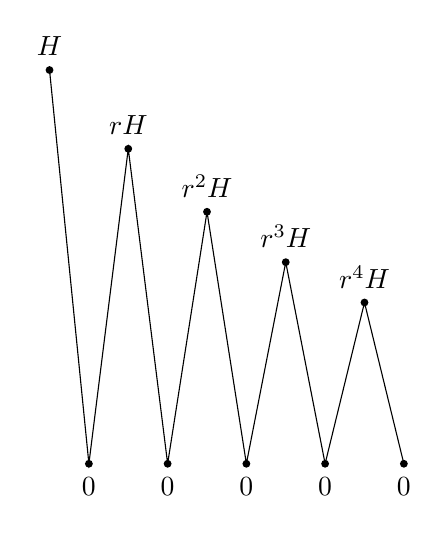
\begin{tikzpicture}[baseline=(current bounding box.north)]
	\draw
	(0,5) node[circle,fill,inner sep=1pt,label=above:$H$](){}
	-- (0.5,0) node[circle,fill,inner sep=1pt,label=below:$0$](){}
	-- (1,4) node[circle,fill,inner sep=1pt,label=above:$rH$](){}
	-- (1.5,0) node[circle,fill,inner sep=1pt,label=below:$0$](){}
	-- (2,3.2) node[circle,fill,inner sep=1pt,label=above:$r^2H$](){}
	-- (2.5,0) node[circle,fill,inner sep=1pt,label=below:$0$](){}
	-- (3,2.56) node[circle,fill,inner sep=1pt,label=above:$r^3H$](){}
	-- (3.5,0) node[circle,fill,inner sep=1pt,label=below:$0$](){}
	-- (4,2.048) node[circle,fill,inner sep=1pt,label=above:$r^4H$](){}
	-- (4.5,0) node[circle,fill,inner sep=1pt,label=below:$0$](){}
	;

\end{tikzpicture}
\parbox[t]{\linewidth-4.5cm}{
	(Of course the ball would not actually move to the right like
	in this diagram - it would only travel the vertical distance
	indicated)

	Let ${b_n}$ be the height of the ball before the $n$th bounce.
	It is a geometric sequence with common ratio $d$ and first term
	$b_1=H$. Let $D$ be the total distance traveled by the ball.
	\begin{align*}
		D&=b_1+b_2+b_2+b_3+b_3+\hdots \\
		D&=\sum_{k=1}^{\infty}b_k+\sum_{k=2}^{\infty}b_k \\
		D&=2\sum_{k=1}^{\infty}b_k-b_1 \\
		D&=2\left(\frac{H}{1-r}\right)-H \\
		\frac{D+H}{2}&=\frac{H}{1-r} \\
		(1-r)\left(\frac{D+H}{2}\right)&=H \\
		1-r&=\frac{2H}{D+H} \\
		r&=\frac{D+H}{D+H}-\frac{2H}{D+H} \\
		\Aboxed{r&=\frac{D-H}{D+H}} \\
	\end{align*}
}

\section*{Problem 6}
\centering
\begin{minipage}[t]{0.3\linewidth}
\begin{align*}
	r=\frac{\sqrt{3}\tan\theta}{\sqrt{2}\sin\theta}&=
		\frac{\sqrt{2}\sin\theta}{\cos\theta} \\
	\frac{\sqrt{3}\tan\theta}{\sqrt{2}\sin\theta}\cdot\cos\theta&=
		\frac{\sqrt{2}\sin\theta}{\cos\theta}\cdot\cos\theta \\
	\frac{\sqrt{3}\sin\theta}{\sqrt{2}\sin\theta}&=
		\sqrt{2}\sin\theta \\
	\frac{\sqrt{3}}{\sqrt{2}}&=\sqrt{2}\sin\theta \\
	2\sin\theta&=\sqrt{3} \\
	\sin\theta&=\frac{\sqrt{3}}{2} \\
	\theta&=\frac{\pi}{3}
\end{align*}
\end{minipage}
\begin{minipage}[t]{0.25\linewidth}
\begin{align*}
	r&=\frac{\sqrt{2}\sin\frac{\pi}{3}}{\cos\frac{\pi}{3}} \\
	r&=\frac{\sqrt{2}\cdot\frac{\sqrt{3}}{2}}{\frac{1}{2}} \\
	r&=\sqrt{2}\cdot\frac{\sqrt{3}}{2}\cdot2 \\
	r&=\sqrt{6} \\
	\\
	a_1&=\frac{\cos\frac{\pi}{3}}{\sqrt{6}} \\
	a_1&=\frac{\frac{1}{2}}{\sqrt{6}} \\
	a_1&=\frac{1}{2\sqrt{6}} \\
\end{align*}
\end{minipage}
\begin{minipage}[t]{0.25\linewidth}
\begin{align*}
	S_6&=a_1\left(\frac{1-r^6}{1-r}\right) \\
	S_6&=\frac{1}{2\sqrt{6}}\left(
			\frac{1-(\sqrt{6})^6}{1-\sqrt{6}}\right) \\
	S_6&=\frac{1-6^3}{2\sqrt{6}-12} \\
	S_6&=\frac{-215}{2\sqrt{6}-12}\cdot
		\frac{2\sqrt{6}+12}{2\sqrt{6}+12} \\
	S_6&=\frac{-430\sqrt{6}-2580}{24-144} \\
	S_6&=\frac{430\sqrt{6}+2580}{144-24} \\
	S_6&=\frac{43\sqrt{6}+258}{12} \\
	\Aboxed{S_6&=\frac{43(6+\sqrt{6})}{12}} \\
\end{align*}
\end{minipage}
\flushleft
\end{document}
